\documentclass{article}
\usepackage{graphicx}
\usepackage{geometry}
\usepackage{enumitem}
\usepackage{hyperref}
\usepackage{listings}
\usepackage{xcolor}

\definecolor{codegreen}{rgb}{0,0.6,0}
\definecolor{codegray}{rgb}{0.5,0.5,0.5}
\definecolor{codepurple}{rgb}{0.58,0,0.82}
\definecolor{backcolour}{rgb}{0.95,0.95,0.92}

\lstdefinestyle{mystyle}{
    backgroundcolor=\color{backcolour},   
    commentstyle=\color{codegreen},
    keywordstyle=\color{magenta},
    numberstyle=\tiny\color{codegray},
    stringstyle=\color{codepurple},
    basicstyle=\ttfamily\footnotesize,
    breakatwhitespace=false,         
    breaklines=true,                 
    captionpos=b,                    
    keepspaces=true,                 
    numbers=left,                    
    numbersep=5pt,                  
    showspaces=false,                
    showstringspaces=false,
    showtabs=false,                  
    tabsize=2
}

\lstset{style=mystyle}

\geometry{a4paper, margin=1in}

\title{Lab Report: Scientific Calculator Using 6×6 Button Matrix}
\author{Dhawal\\ ee24btech11015}

\begin{document}

\maketitle

\section{Aim}
To design and implement a scientific calculator using:
\begin{itemize}
    \item Arduino microcontroller
    \item 6×6 button matrix for input
    \item 16×2 LCD display for output
    \item Advanced mathematical functions (trigonometric, logarithmic, etc.)
\end{itemize}

\section{Materials Required}
\subsection{Hardware Components}
\begin{itemize}
    \item Arduino Uno board
    \item 6×6 button matrix (36 buttons total)
    \item 16×2 LCD display
    \item 10k ohm resistors (for pull-up)
    \item Breadboard and jumper wires
    \item Potentiometer (for LCD contrast adjustment)
\end{itemize}

\subsection{Software}
\begin{itemize}
    \item Arduino IDE
    \item AVR GCC compiler
    \item Custom libraries: parser.h, funcs.h
\end{itemize}

\section{Circuit Connections}

\subsection{LCD Connections}
\begin{itemize}
    \item \textbf{Control Pins}:
    \begin{itemize}
        \item RS to PB0
        \item E to PB1
        \item RW to GND
    \end{itemize}
    \item \textbf{Data Pins}:
    \begin{itemize}
        \item DB4 to PB2
        \item DB5 to PB3
        \item DB6 to PB4
        \item DB7 to PB5
    \end{itemize}
\end{itemize}

\subsection{Button Matrix Connections}
\begin{itemize}
    \item \textbf{Rows} (Outputs):
    \begin{itemize}
        \item Rows 1-6 to PC0-PC5
    \end{itemize}
    \item \textbf{Columns} (Inputs with pull-ups):
    \begin{itemize}
        \item Columns 1-6 to PD2-PD7
    \end{itemize}
\end{itemize}

\section{System Design}

\subsection{Button Matrix Layout}
The 6×6 matrix is organized into two modes:

\begin{table}[h]
\centering
\begin{tabular}{|l|l|l|l|l|l|}
\hline
\textbf{Basic Mode} & \multicolumn{5}{c|}{\textbf{Button Functions}} \\
\hline
0-9 & Basic numbers &  &  &  &  \\
\hline
(, ) & Parentheses & f & s (sin) & c (cos) & t (tan) \\
\hline
+,-,*,/ & Basic ops & \^{} (pow) & ! (fact) &  &  \\
\hline
= & Equals & . & \_ (clear) & < (back) & \& (mode) \\
\hline
@ (asin) & \# (acos) & \$ (atan) & l (ln) & e & p ($\pi$) \\
\hline
\end{tabular}
\end{table}

\begin{table}[h]
\centering
\begin{tabular}{|l|l|l|l|l|l|}
\hline
\textbf{Advanced Mode} & \multicolumn{5}{c|}{\textbf{Button Functions}} \\
\hline
0-9 & Basic numbers &  &  &  &  \\
\hline
m (mem store) & M (mem recall) & @ & \# & \$ & : (tanh) \\
\hline
! & e & p & \% & l & ( \\
\hline
= & . & \_ & < & \& & ) \\
\hline
s & c & t & , (sinh) & ? (cosh) & : (tanh) \\
\hline
\end{tabular}
\end{table}

\section{Key Features}

\subsection{Mathematical Functions}
\begin{itemize}
    \item Basic arithmetic (+, -, *, /)
    \item Trigonometric (sin, cos, tan)
    \item Hyperbolic (sinh, cosh, tanh)
    \item Inverse trigonometric (asin, acos, atan)
    \item Logarithmic (ln)
    \item Power and factorial (x\^{}y, x!)
    \item Memory functions (store/recall)
    \item Fraction conversion
\end{itemize}

\subsection{Display System}
\begin{itemize}
    \item Two-line 16-character LCD
    \item Top line shows current expression
    \item Bottom line shows results
    \item Special character support ($\pi$, fractions)
    \item Scientific notation for large numbers
\end{itemize}

\section{Implementation Details}

\subsection{Key Algorithms}
\begin{enumerate}
    \item \textbf{Button Scanning}:
    \begin{itemize}
        \item Rows are set low sequentially
        \item Columns are read to detect presses
        \item Debouncing implemented in software
    \end{itemize}
    
    \item \textbf{Expression Evaluation}:
    \begin{itemize}
        \item Custom parser handles operator precedence
        \item Supports nested parentheses
        \item Converts button codes to mathematical operations
    \end{itemize}
    
    \item \textbf{Display Handling}:
    \begin{itemize}
        \item Special encoding for functions (sin to 's')
        \item Automatic scrolling for long expressions
        \item Dual-line display management
    \end{itemize}
\end{enumerate}

\section{Observations}
\begin{center}
        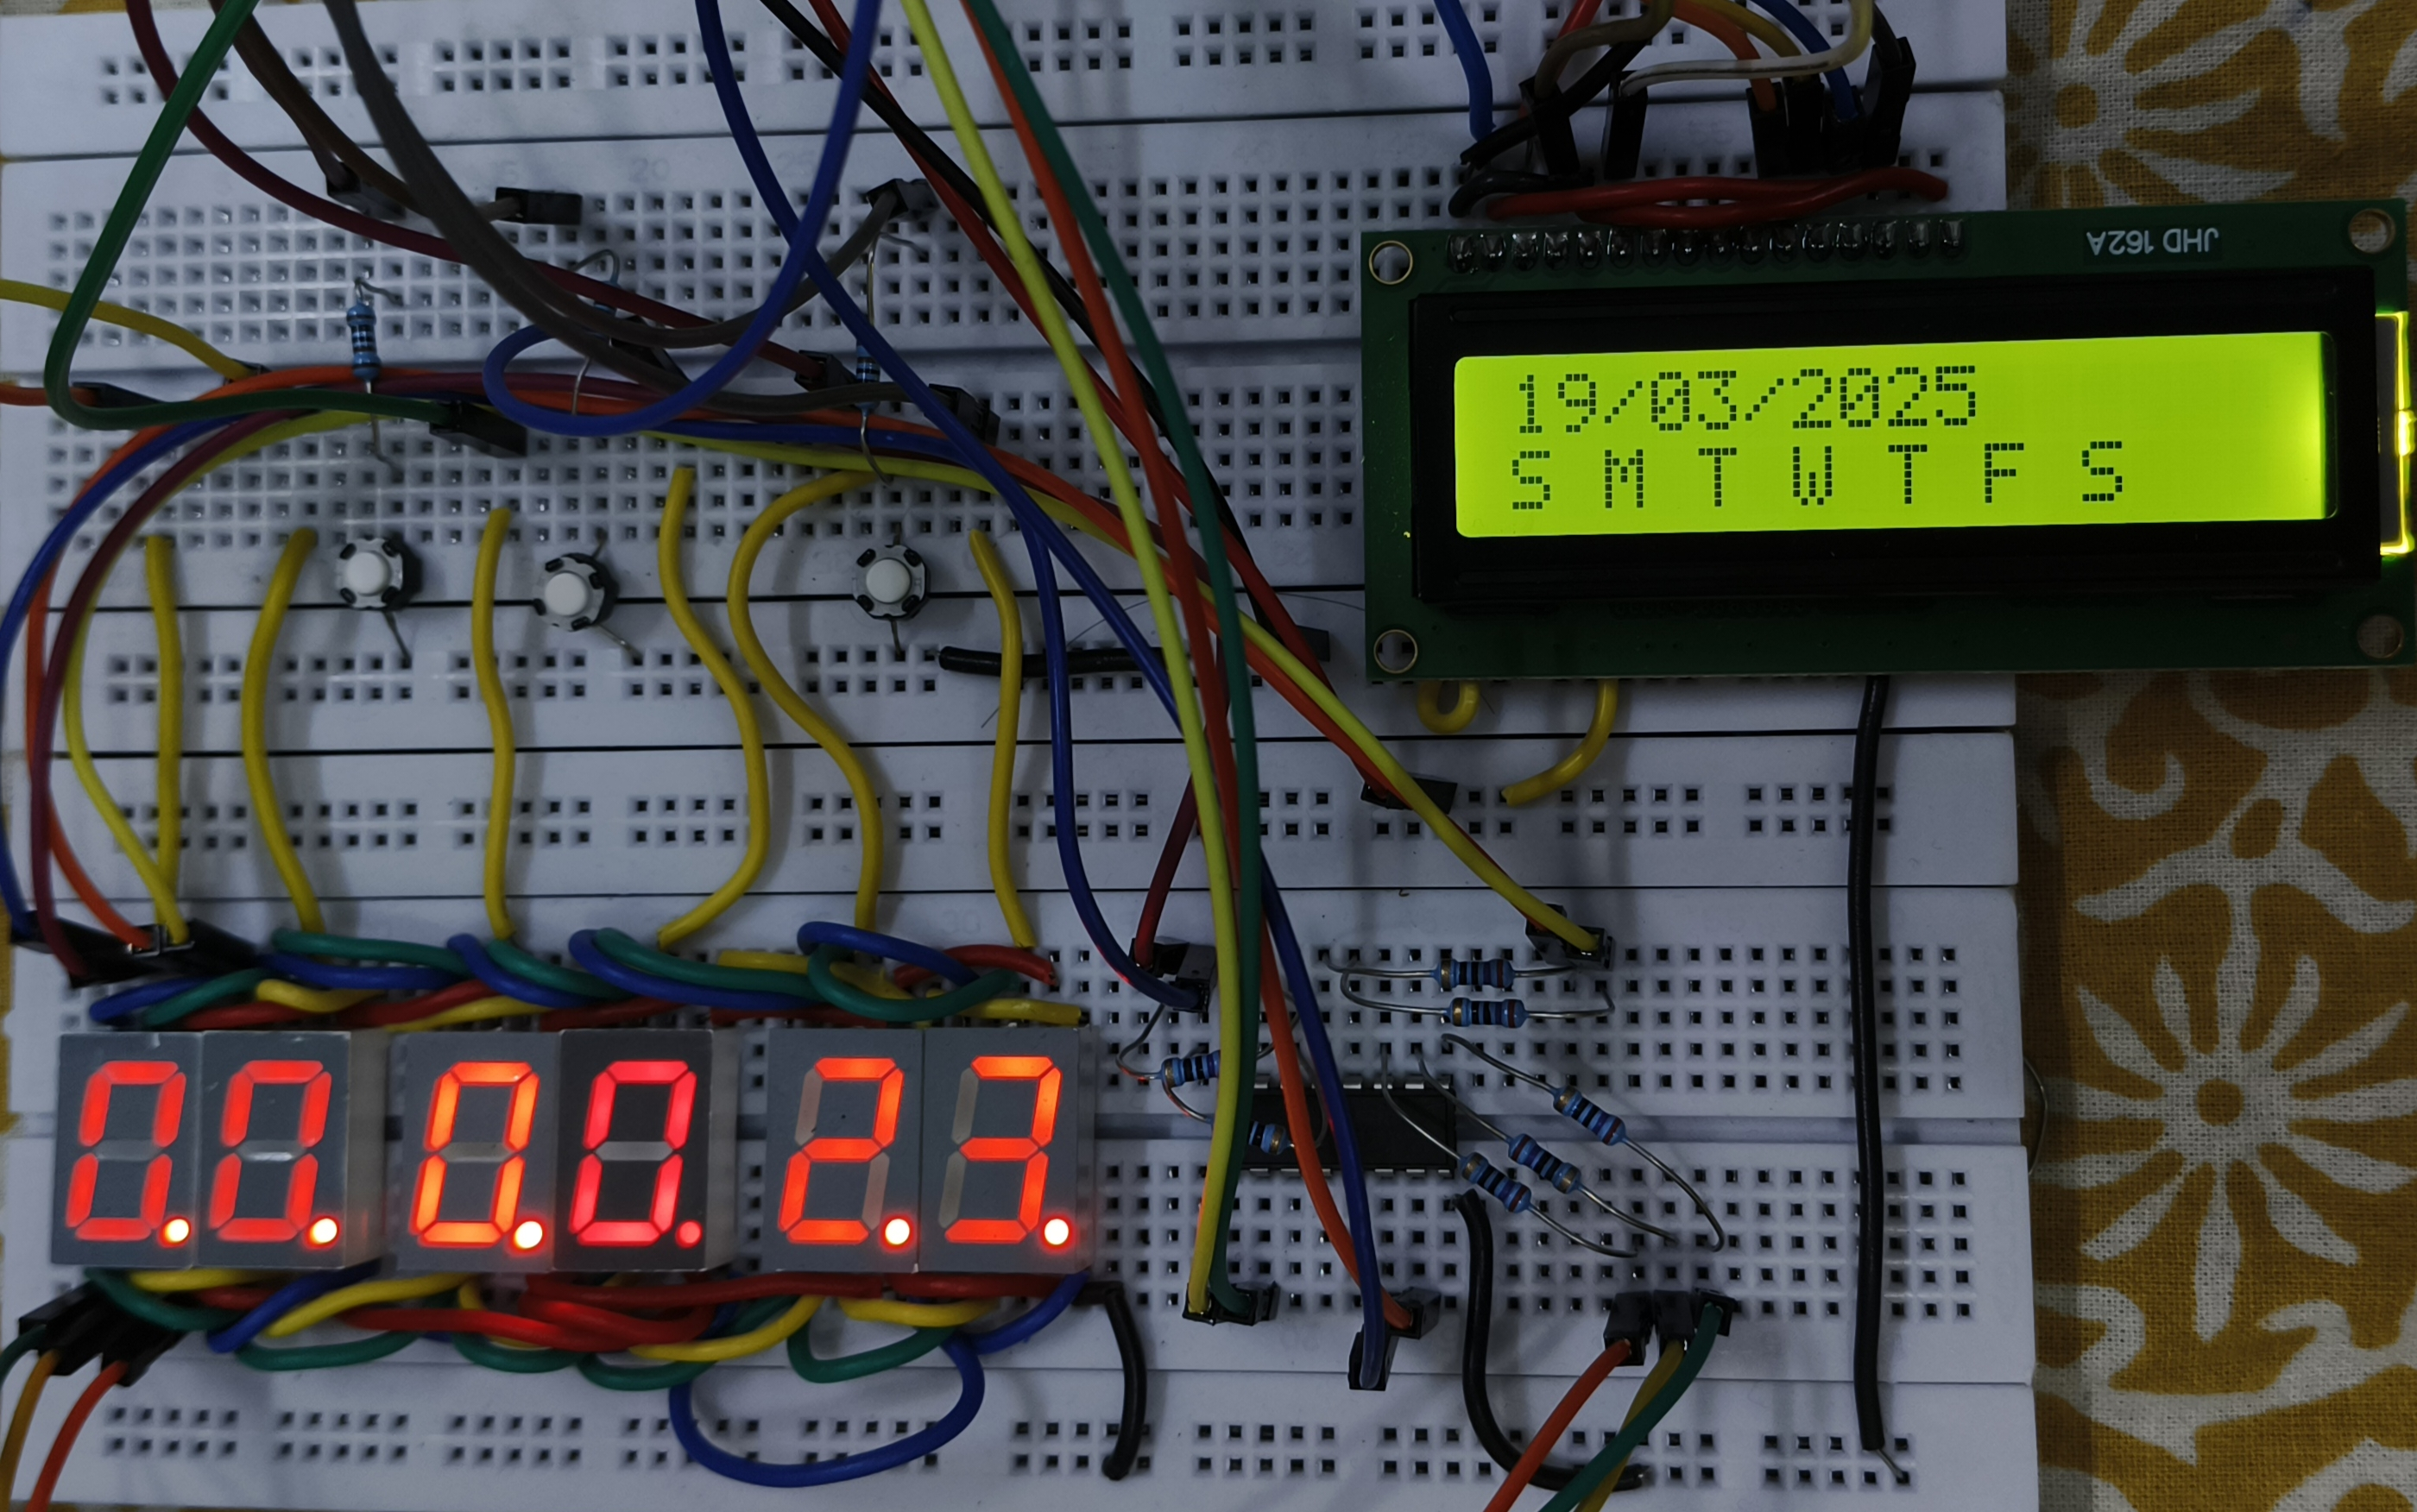
\includegraphics[width=0.5\textwidth]{figs/1.jpg}
    \end{center}
\subsection{Basic Operation}
\begin{itemize}
    \item System boots with "Calculator ready" message
    \item Buttons respond within 50ms debounce period
    \item Results display with 5 decimal places precision
    \item Automatic mode switching works reliably
\end{itemize}

\subsection{Performance Metrics}
\begin{itemize}
    \item \textbf{Scan Rate}: 50Hz button matrix scan
    \item \textbf{Response Time}: <100ms for basic operations
    \item \textbf{Accuracy}: IEEE 754 double precision
    \item \textbf{Memory}: Uses EEPROM for value storage
\end{itemize}

\section{Challenges and Solutions}

\subsection{Button Ghosting}
\begin{itemize}
    \item \textbf{Problem}: False presses in matrix
    \item \textbf{Solution}: Implemented sequential scanning with pull-ups
\end{itemize}

\subsection{Display Limitations}
\begin{itemize}
    \item \textbf{Problem}: Limited 16×2 display space
    \item \textbf{Solution}: Implemented scrolling and abbreviation
\end{itemize}

\subsection{Precision Issues}
\begin{itemize}
    \item \textbf{Problem}: Floating point errors
    \item \textbf{Solution}: Used double precision and proper rounding
\end{itemize}

\section{Conclusion}
The scientific calculator successfully implements:
\begin{itemize}
    \item Comprehensive mathematical operations
    \item Efficient button matrix scanning
    \item Clear display output
    \item Multiple operation modes
\end{itemize}


\end{document}
